% Drawing 146/04-1 -- folder 146, batch 04, archive page 61 (PDF page 62).
% Transcription: En tête de page, plusieurs croquis : un octaèdre (ou double pyramide) aux faces hachurées ; un triangle avec un petit triangle intérieur ; deux triangles réunis par un sommet (« nœud papillon ») ; un triangle marqué $+$, avec au-dessous un segment et un triangle aux sommets $0$, $1$, $\infty$.
% Kind: small polyhedral sketches. Method 2 (schematic redraw from the facsimile). Status: ok.
% Notes: Octahedron / double pyramid with two hatched faces (its apex touches the top edge of the bbox); a triangle with a small inner triangle; the bow-tie (two triangles sharing a vertex); a triangle marked + with an inner vertex, a segment with three points, and the triangle 0, 1, infinity (only its strokes; the labels are placed from the transcription, their exact attribution to the corners uncertain). A small mark under the second triangle (a « 4 »?) is not read and left out.
% Coordinates: 1 unit = 1 mm = 1/100 of the crop width (bbox in page fractions: [0.27, 0.1, 0.71, 0.245]).
% Redrawn by Claude (claude-opus-5-5), issue #73 pilot, 2026-11-07; not checked by a human; not compiled (no TeX in the session).
% Rights: reproduces part of the work -- behind RENDER_TRANSCRIPTS, never published by itself.
\documentclass[tikz,border=3pt]{standalone}
\usepackage{amsmath,amssymb}
\usetikzlibrary{patterns,arrows.meta}
\tikzset{pencil/.style={black!45}, struck/.style={black!35}, mark/.style={circle,draw,inner sep=1.3pt}, pt/.style={circle,fill,inner sep=0.9pt}, opt/.style={circle,draw,fill=white,inner sep=1.1pt}}
\begin{document}
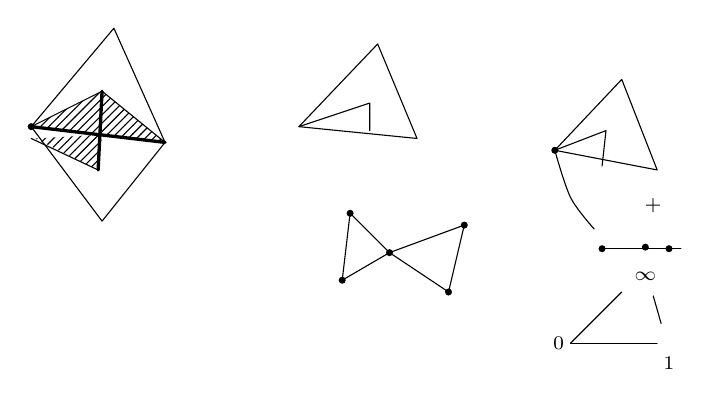
\begin{tikzpicture}[x=1mm,y=1mm,line cap=round,line join=round,font=\scriptsize]
\draw (23,-0.5) -- (12.5,-13) -- (21.5,-25) -- (29.5,-15) -- cycle;
\draw[very thick] (12.5,-13) -- (29.5,-15);
\draw (12.5,-13) -- (21.5,-8.5) -- (29.5,-15);
\draw[very thick] (21.5,-8.5) -- (21,-18.5);
\draw (12.5,-14.5) -- (21,-18.5);
\fill[pattern=north east lines] (12.5,-13) -- (21.5,-8.5) -- (21.5,-14) -- cycle;
\fill[pattern=north east lines] (13,-14.5) -- (21,-18.5) -- (21.5,-14) -- cycle;
\fill[pattern=north east lines] (21.5,-8.5) -- (29.5,-15) -- (21.5,-14) -- cycle;
\node[pt] at (12.5,-13) {};
\draw (46.5,-13) -- (56.5,-2.5) -- (61.5,-14.5) -- cycle;
\draw (46.5,-13) -- (55.5,-10) -- (55.5,-13.5);
\draw (53,-24) -- (52,-32.5) -- (58,-29) -- cycle;
\draw (58,-29) -- (67.5,-25.5) -- (65.5,-34) -- cycle;
\node[pt] at (53,-24) {};
\node[pt] at (52,-32.5) {};
\node[pt] at (58,-29) {};
\node[pt] at (67.5,-25.5) {};
\node[pt] at (65.5,-34) {};
\draw (79,-16) -- (87.5,-7) -- (92,-18.5) -- cycle;
\draw (79,-16) -- (85.5,-13.5) -- (85,-18);
\draw plot[smooth, tension=0.55] coordinates {(79,-16) (81,-22) (84,-26)};
\node[pt] at (79,-16) {};
\node[inner sep=1pt] at (91.5,-23) {\scriptsize $+$};
\draw (85,-28.5) -- (95,-28.5);
\node[pt] at (85,-28.5) {};
\node[pt] at (90.5,-28.3) {};
\node[pt] at (93.5,-28.5) {};
\draw (81,-40.5) -- (87.5,-34);
\draw (81,-40.5) -- (92,-40.5);
\draw (91.5,-34.5) -- (92.5,-38);
\node[inner sep=1pt] at (79.5,-40.5) {\scriptsize $0$};
\node[inner sep=1pt] at (90.5,-32) {\scriptsize $\infty$};
\node[inner sep=1pt] at (93.5,-43) {\scriptsize $1$};
\end{tikzpicture}
\end{document}
